%%%%%%%%%%%%%%%%%%%%%%%%%%%%%%%%%%%%%%%%%%%%%%%%%%%%%%%%%%%%%%%%%%%%
% This is a thesis template for Gebze Technical University.
%
% Please only edit the areas proceeded by a comment starting with %%
% otherwise the template may be broken.
%
% This file is only to be used for editing the general fields
% and inputting the body of the thesis in the designated areas.
% Please write the body of the thesis in separate files, and input
% them as shown in the comment preceding the area.
%
% Created in Aug 2021 by Usama Derbashi.
%%%%%%%%%%%%%%%%%%%%%%%%%%%%%%%%%%%%%%%%%%%%%%%%%%%%%%%%%%%%%%%%%%%%
\documentclass[12pt]{report}


% Language and typeset setting
\usepackage[english]{babel}
\usepackage[a4paper,top=25mm,bottom=25mm,left=40mm,right=25mm]{geometry}
\usepackage[onehalfspacing]{setspace}
\usepackage{indentfirst}
\setlength{\parindent}{1cm}
\setlength{\abovecaptionskip}{12pt plus 0pt minus 0pt}
\setlength{\belowcaptionskip}{12pt plus 0pt minus 0pt}
\setlength{\textfloatsep}{18.0pt plus 0.0pt minus 0.0pt}
\setlength{\floatsep}{18.0pt plus 0.0pt minus 0.0pt}
\setlength{\intextsep}{18.0pt plus 0.0pt minus 0.0pt}
\setlength{\skip\footins}{18.0pt plus 0.0pt minus 0.0pt}

% Core packages and settings
\usepackage[colorlinks=false]{hyperref}
\usepackage{amsmath}

\usepackage{titlesec} %setting the titles of chapters and sections
\setcounter{secnumdepth}{4}
\setcounter{tocdepth}{4}
\titleformat{\chapter}[hang]{\normalfont\bfseries\MakeUppercase}{}{0pt}{\LARGE\thechapter. }
\titleformat{\section}[hang]{\normalfont\bfseries}{}{0pt}{\Large\thesection. }
\titleformat{\subsection}[hang]{\normalfont\bfseries}{}{0pt}{\large\thesubsection. }
\titleformat{\subsubsection}[hang]{\normalfont\bfseries}{}{0pt}{\large\thesubsubsection. }
\titlespacing*{\chapter}{0pt}{0pt}{18pt}
\titlespacing*{\section}{0pt}{18pt}{18pt}
\titlespacing*{\subsection}{0pt}{18pt}{18pt}
\titlespacing*{\subsubsection}{0pt}{18pt}{18pt}

\usepackage{graphicx}
\graphicspath{{./Imgs/}} %pointing the directory of images

\usepackage{fancyhdr} % setting footers
\usepackage{etoolbox} 
\renewcommand{\headrulewidth}{0pt}
\patchcmd{\chapter}{\thispagestyle{plain}}{\thispagestyle{fancy}}{}{}
\pagestyle{fancy}
\fancyhf{}
\fancyfoot[C]{\fontsize{11pt}{11pt}\thepage}

\usepackage[style=ieee]{biblatex}
\addbibresource{refs.bib}
\usepackage{csquotes}% Needed for babel(in biblatex)

\usepackage[bottom, perpage]{footmisc}%% amkes footnotes at the bottom

\usepackage{GTUThesis}


% Additional packages if needed
%% For the sake of not messing the template add them here
\usepackage{lipsum}


% Important information
%% Make sure to enter all the info below
\title{The testing of the new template}
\author{Usama Derbashi}
\faculty{Faculty of Engineering}
\department{Testing Software}
\project{Demonstrative Work}
\supervisor{Prof. Zafeirakis Zafeirakopoulos}
\theyear{2021}


\begin{document}

%Front Matter
\pagenumbering{roman} %start with roman numbering 
\maketitle
\setcounter{page}{3} %the first two title pages are not counted so this is a buffer
\begin{outertitles} % makes titles centred

%% below enter as follows 
%% {DECREE_NO}{DATE_OF_DECREE}{DATE_OF_DEFENCE}{JURY}
%% Note that JURY should be comma separated
%% note that if there is no decree DECREE_NO and DATE_OF_DECREE left empty
\makejury{2021/314}{31/04/2021}{31/08/2021}{Prof. Erchan Aptoula, M.Sc Melike Ilteralp}

\chapter*{Abstract}
\addcontentsline{toc}{chapter}{Abstract}

%% Edit below this line
Somebody once told me the world is gonna roll me; I ain't the sharpest tool in the shed.

She was looking kind of dumb with her finger and her thumb, in the shape of an "L" on her forehead.

Well, the years start coming and they don't stop coming.

Fed to the rules and I hit the ground running.

Didn't make sense not to live for fun, your brain gets smart but your head gets dumb.

So much to do, so much to see, so what's wrong with taking the back streets?

You'll never know if you don't go.

You'll never shine if you don't glow.

Hey, now, you're an all-star, get your game on, go play!

Hey, now, you're a rock star, get the show on, get paid!

And all that glitters is gold, only shooting stars break the mold.

It's a cool place and they say it gets colder.

You're bundled up now wait 'til you get older.

But the meteor men beg to differ, judging by the hole in the satellite picture.

The ice we skate is getting pretty thin.

The water's getting warm so you might as well swim.

My world's on fire. How about yours?

That's the way I like it and I'll never get bored.

Somebody once asked could I spare some change for gas, I need to get myself away from this place.

I said yep, what a concept! I could use a little fuel myself! And we could all use a little change!


%% Until here
\vfill
%% Edit after {Keywords:}
\textbf{Keywords:} All-Star, Smash Mouth, Shrek, Change, Hope.
\clearpage
\chapter*{Özet}
\addcontentsline{toc}{chapter}{Özet}

%% Edit below this line
Bir keresinde biri bana dünyanın beni yuvarlayacağını söylemişti; Ben kulübedeki en keskin alet değilim.

Alnında "L" şeklinde parmağı ve baş parmağıyla biraz aptal görünüyordu.

Eh, yıllar gelmeye başlar ve gelmekten vazgeçmezler.

Kurallara uydum ve koşarak yere vurdum.

Eğlenmek için yaşamamak anlamsızdı, beynin akıyor ama kafan aptallaşıyor.

Yapacak çok şey, görülecek çok şey var, peki arka sokaklara gitmenin nesi yanlış?

Gitmezsen asla bilemezsin.

Parlamazsan asla parlayamazsın.

Hey, şimdi, sen bir yıldızsın, oyununa başla, git oyna!

Hey, şimdi, sen bir rock yıldızısın, şovu başlat, paranı al!

Ve parıldayan her şey altındır, yalnızca kayan yıldızlar kalıbı kırar.

Serin bir yer ve soğuduğunu söylüyorlar.

Artık toplandınız, yaşlanana kadar bekleyin.

Ancak meteor adamları, uydu resmindeki deliğe bakılırsa, farklı olmak için yalvarıyorlar.

Kaydırdığımız buz oldukça inceliyor.

Su ısınıyor, bu yüzden yüzebilirsin.

Dünyam yanıyor. Ya sizinkiler?

Bu benim hoşuma gidiyor ve asla sıkılmayacağım.

Biri bir keresinde benzin için biraz para ayırabilir miyim diye sordu, kendimi buradan uzaklaştırmalıyım.

Evet dedim, ne konsept! Ben de biraz yakıt kullanabilirim! Ve hepimiz biraz değişiklik yapabiliriz!

%% Until here
\vfill
%% Edit after {Anahtar Kelimeler:}
\textbf{Anahtar Kelimeler:} Tüm-Yıldız, Ağız Parçalamak, Shrek, Değişim, Umut.
\clearpage
\ifbool{isEN}{%
    \chapter*{Acknowledgement}
    \addcontentsline{toc}{chapter}{Acknowledgement}
}{
    \chapter*{Teşekkür}
    \addcontentsline{toc}{chapter}{Teşekkür}
}
%% Edit below this line
Thank you mate!!

%% Until here
\clearpage
\ifbool{isEN}{%
    \chapter*{List of Symbols and Abbreviations}
    \addcontentsline{toc}{chapter}{List of Symbols and Abbreviations}
}{
    \chapter*{Simgeler ve Kısaltmalar Dizini}
    \addcontentsline{toc}{chapter}{Simgeler ve Kısaltmalar Dizini}
}

\begin{tabular}{lcl}
    \ifbool{isEN}{%
        \underline{\textbf{Symbol or}}&&\\
        \underline{\textbf{Abbreviation}} &:& \underline{\textbf{Explanation}}\\
    }{
        \underline{\textbf{Simgeler ve}}&&\\
        \underline{\textbf{Kısaltmalar}} &:& \underline{\textbf{Açıklamalar}}\\
    }
    
    %% Edit below in the format
    %% XYZ &:& EXPLANATION\\
    %% where XYZ is the acronym or symbol
    %% and EXPLANATION is the explanation of it
    %% make sure not to forget &:& between them, and \\ at the end of EXPLANATION
    
    BM &:& Back-matter\\
    FM &:& Front-matter\\
    MM &:& Main-matter\\
    
    %% Until here
\end{tabular}

\clearpage

\tableofcontents
\addcontentsline{toc}{chapter}{Contents}
\clearpage

\listoffigures
\addcontentsline{toc}{chapter}{List of Figures}
\clearpage

\listoftables
\addcontentsline{toc}{chapter}{List of Tables}
\clearpage

\end{outertitles}
\fancyhf{}%reset footer
\fancyfoot[R]{\fontsize{11pt}{11pt}\thepage}%page numbers in the corner
\addtocontents{toc}{\protect\vspace{18pt}}
\pagenumbering{arabic}%turn to arabic numbers

% Mainmatter

%% Only input files, don't write here
%% \input{./Body/Mainmatter/FILE}
\chapter{Usage}

\section{Project Structure}

In order to use the project more efficiently I thought an explanation of the structure of the project would be a good place to start to further the understanding of the different elements of the project. \Cref{fig:struct} shows the structure.

\begin{figure}
    \centering
    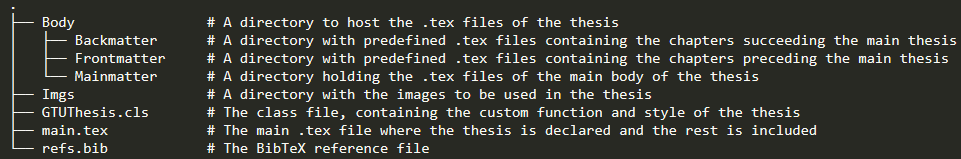
\includegraphics[width=\linewidth]{struct}
    \caption{The structure of the project, if too small please refer to the Github repo\cite{github}}
    \label{fig:struct}
\end{figure}


\section{Backmatter and Frontmatter}

As mentioned in the structure, these directories (\texttt{./Body/Backmatter} and \texttt{./Body/Frontmatter}) contain \texttt{.tex} files with the chapters preceding and succeeding the main body of the thesis, like abstract, list of acronyms, and appendices. The comments in the files themselves indicate where and what to write. Please don't edit the areas not meant to be edited.

\section{Mainmatter}\label{sec:mainmatter}

The \texttt{./Body/Mainmatter} directory is to house the \texttt{.tex} files of the main body of the thesis to be later included in the \texttt{./main.tex} (see \Cref{sec:maintex}). They can be named anything and organised within the directory in any way deemed fit. The example has two files (\texttt{C1.tex} and \texttt{C2.tex}) demonstrating a way of using the files, but it can be used in any other way, name or convention deemed appropriate by the user.

\section{Imgs and refs.bib}

As mentioned in the structure, \texttt{./Imgs} is a directory to house the images to be used in the figures of the thesis. The files in the directory could be further organised into subdirectories, but the file \texttt{./Imgs/gtu\_logo.jpg} to stay in its place.

As for \texttt{refs.bib}, this is a BibTeX file to be filled in with the references to be used for the thesis. (copied from the publisher or scholar.google.com)

\section{GTUThesis.cls}\label{sec:cls}

This is the file containing the custom functions and style of the GTU thesis. See \Cref{ch:class} for the documentation. \textbf{\textit{DO NOT}} modify this file unless you know what you're doing and sure about the changes you want to do.

\section{main.tex}\label{sec:maintex}

This is the main \texttt{.tex} file where the user firstly declares the document class as \texttt{GTUThesis} and then fills in the GTU-fields, followed by the used packages, and then starts the document environment, where they are expected to call the \texttt{GTUMakeFront} and \texttt{GTUMakeBack} functions respectively right after the start and before the end of the document environment. See \Cref{ch:class} for the documentation.

Between the \texttt{GTUMakeFront} and \texttt{GTUMakeBack} functions the user can include the files of the Main matter (recommended, see \Cref{sec:mainmatter}) using the include function as follows:

	\texttt{~~~~\textbackslash include\{./Body/Mainmatter/FILE.tex\}}

or write their thesis in the way they see fitting.

\section{Important Note}

\textbf{\textit{DO NOT}} delete, rename, or move the following files or directories because their paths are hard-coded:
\begin{itemize}
    \item \texttt{./Body}
    \item \texttt{./Body/Backmatter}
    \item \texttt{./Body/Backmatter/Appendices.tex}
    \item \texttt{./Body/Backmatter/CV.tex}
    \item \texttt{./Body/Frontmatter}
    \item \texttt{./Body/Frontmatter/Abstract.tex}
    \item \texttt{./Body/Frontmatter/Acknowledgement.tex}
    \item \texttt{./Body/Frontmatter/ListOfAcro.tex}
    \item \texttt{./Body/Frontmatter/Ozet.tex}
    \item \texttt{./Imgs}
    \item \texttt{./Imgs/gtu\_logo.jpg}
    \item \texttt{./GTUThesis.cls}
    \item \texttt{./refs.bib}
\end{itemize}
\chapter{GTUThesis Class} \label{ch:class}

\texttt{GTUThesis.cls} (see \Cref{sec:cls}) is the star of the show here, where the style of the thesis of GTU is defined. The user is expected to use some functions, and the demo \texttt{main.tex} shows how it is used. But for the sake of completion,  here is the documentation for the functions which the user is expected to call in their main.

\section{Declare Class}\label{sec:declare}

	\texttt{~~~~\textbackslash documentclass[lang,degree]\{GTUThesis\}}

The \texttt{lang} and \texttt{degree} options are set to set the language of the thesis (including titles and predefined text), and the degree which mainly changes some slight things in the Frontmatter. \texttt{lang} can take either \texttt{en} or \texttt{tr} with the former being the default, and \texttt{degree} takes either \texttt{undergrad} or \texttt{graduate} with the latter being the default.

\section{GTU Fields}

These are the fields required to be filled in at the beginning of the documents, they all take one argument in the following matter

	\texttt{~~~~\textbackslash GTUField\{argument\}}

and they are the following.

\begin{table}
    \caption{GTU-fields and their arguments}
    \label{tab:fields}
    \centering
    \begin{tabular}{|l|l|l|}
        \hline
        \textbf{GTU Field} & \textbf{Taken Argument} \\
        \hline
        GTUAuthor & Name of the author of the thesis (student)\\
        GTUTitle & The title of the thesis\\
        GTUFaculty & The faculty or institute of the author\\
        GTUDepartment & The department of the author\\
        GTUProject & The project the author is working on (ex. PhD thesis)\\
        GTUSupervisor & Name of the supervisor\\
        GTUYear & The year of the publication of the thesis\\
        GTUJury & Names of the jury for the thesis (comma separated) \\
        GTUDefenceDate & The date when the author presents the project to the jury\\
        GTUDecreeNo & The decree number of the jury formation (only graduate)\\
        GTUDecreeDate & The above decree's date (only graduate)\\
        \hline
    \end{tabular}
\end{table}


\section{GTU Make}

These are two functions which produce the front-matter and the back-matter of the thesis.

	\texttt{\textbackslash GTUMakeFront}

The function above produces the front-matter including the cover, the lists of content, figures, tables, and acronyms etc. in the correct order and in the correct format for the declared class's arguments (see \Cref{sec:declare} for more).

	\texttt{\textbackslash GTUMakeBack\{arg\}}

The function above produces the back-matter including the bibliography, and the optional CV and appendices. \texttt{arg} is a string that takes in the optional sections which the user wants to add comma separated (\texttt{cv} for the CV and \texttt{ap} for the appendices). If the user still doesn't want any optional sections, they still have to add the empty \texttt{\{\}} since the function waits for an argument which can be an empty string. So, the valid uses of the function are 

	\texttt{\textbackslash GTUMakeBack\{\} \% for only bibliography}
	
	\texttt{\textbackslash GTUMakeBack\{cv\} \% for bibliography and CV}
	
	\texttt{\textbackslash GTUMakeBack\{ap\} \% for bibliography and appendices}
	
	\texttt{\textbackslash GTUMakeBack\{cv,ap\} \% for bibliography, CV, and appendices}

\section{A Section to catch some other things}


Let $X_1, X_2, \ldots, X_n$ be a sequence of independent and identically distributed random variables with $\text{E}[X_i] = \mu$ and $\text{Var}[X_i] = \sigma^2 < \infty$, and let
\begin{equation}
    S_n = \frac{X_1 + X_2 + \cdots + X_n}{n}
      = \frac{1}{n}\sum_{i}^{n} X_i
\end{equation}
denote their mean. Then as $n$ approaches infinity, the random variables $\sqrt{n}(S_n - \mu)$ converge in distribution to a normal $\mathcal{N}(0, \sigma^2)$.

\begin{quote}
    \lipsum[10] \footnote{The text in this quote was created with \texttt{lipsum} package}
\end{quote}



% DON'T INPUT FILES AFTER HERE
\begin{outertitles}
\clearpage
\setlength{\emergencystretch}{1em}
\printbibliography
\addtocontents{toc}{\protect\vspace{18pt}}
\addcontentsline{toc}{chapter}{Bibliography}
%% If you don't want a CV or appendices add a % at the beginning of the relevant line
\chapter*{CV}
\addcontentsline{toc}{chapter}{CV}

%% Edit below this line
Hi, my name is, what? My name is, who?
My name is, chka-chka, Slim Shady
Hi, my name is, huh? My name is, what?
My name is, chka-chka, Slim Shady
Hi, my name is, what? (Excuse me) My name is, who?
My name is, chka-chka, Slim Shady
(Can I have the attention of the class for one second?)
Hi, my name is, huh? My name is, what?
My name is, chka-chka, Slim Shady



%% Until here
\clearpage
\ifbool{isEN}{%
    \chapter*{Appendices}
\addcontentsline{toc}{chapter}{Appendices}
}{
    \chapter*{Ekler}
\addcontentsline{toc}{chapter}{Ekler}
}
%% Edit below this line

\section*{Appendix 1: Some publications}

No one significant, in AAA.

\section*{Appendix 2: Some explanation}

None needed mate!
\end{outertitles}
\end{document}